\documentclass[t, notes, xcolor=table]{beamer}

\usepackage{wrapfig}
\usepackage{float}
% For tabs in verbatim
\usepackage{fancyvrb}

% set fonts
\usefonttheme{professionalfonts} % using non standard fonts for beamer
\usepackage{txfonts,mathptmx}

% set indend spacing for first and second level indentation
\setlength{\leftmargini}{0.5cm}
\setlength{\leftmarginii}{0.5cm}
\setlength{\leftmarginiii}{0.5cm}

% Set circles for bullets 
\setbeamertemplate{itemize items}[circle]

% colors
\usepackage{xcolor}

% multiple columns
\usepackage{multicol}

% todo lists
\usepackage{pifont}
\usepackage{amssymb}

% increase space between text and frame name
\addtobeamertemplate{frametitle}{}{\vspace{0.5em}}

%Information to be included in the title page:
\title{Choosing Between Verilog Data Types}
\author{Nikola Petrovic}
\institute{University of Belgrade, School of Electrical Engineering}
\date{2022}



\begin{document}

\frame{\titlepage}

%%%%%%%%%%%%%%%%%%%%%%%%%%%%%%%%%%%%%%%%%%%%%%%%%%%%%%%%%%%%
\begin{frame}
\frametitle{Module Objective}

In this module we will choose and use the Verilog data types correctly.
\newline

\textbf{Topics}

\begin{itemize}
\item Logic values
\item Net and Register type rules and example
\item Declaring vectors (truncation and padding)
\item Defining literal values
\item Declaring nets
\item Declaring variables
\item Declaring arrays of nets and variables
\item Declaring module parameters
\end{itemize}

\end{frame}

%%%%%%%%%%%%%%%%%%%%%%%%%%%%%%%%%%%%%%%%%%%%%%%%%%%%%%%%%%%%
\begin{frame}
\frametitle{Value Set}
\footnotesize{

\begin{tabular}{ |c|l| } 
\hline
 \rowcolor{lightgray} 
 Value & Associated Informal Terms  \\ 
 \hline
 0 & Zero, Low, False, Logic Low, Ground, VSS  \\ 
 \hline
 1 & One, High, True, Logic High, Power, VDD, VCC  \\ 
 \hline
 Z & HiZ, High Impedance, Tri-State, Undriven, Unconnected, Driver disabled   \\ 
 \hline
 X & Uninitialized, Unknown  \\ 
 \hline
\end{tabular}
}
\end{frame}

\note{

\footnotesize{
The Verilog value set consists of four basic values:
\begin{itemize}
\item 0 - Represents a logic zero, low, false condition
\item 1 - Represents a logic one, high, true condition
\item Z - Represents a high impedance state
\item X - Represents an unknown state
\end{itemize}
}
}

\note{

\tiny{
The simulator initializes most nets to high-impedance state. The exception are nets of \textbf{trireg} type, this is because they represents capacitive nets so they are initialized to unknown value.
\newline

Upon commencing the simulation, simulator propagates the values of net drivers onto the nets. A net that has no drivers will remain in its initialized value throughout the simulation. This situation is usually the result of user error, as there are seldom good reason to leave a net undriven.
\newline

The simulator initialized most variables to unknown value. The exception is variable of the \textbf{real} type, which is initialized to 0 since this is the only type that cannot hold high-impedance or unknown values.
\newline

A variable that is never assigned a value will remained in its initialized value throughout simulation.
\newline

The appearance during simulation of a high-impedance value on a net is usually due to its drivers being disabled. In real hardware this situation either has short duration or doesn't occur because bus keepers pull the nets to a high or a low logic states. 
\newline

The appearance during simulation of a unknown value on a net is usually due to clash between drivers driving different values. In real hardware, this situation will either not exist or have an extremely short duration.
\newline

The appearance during simulation of a high-impedance value on a variable is due to the assignment of that value to the variable, either deliberately because that value represents one of the drivers on the bus net, or by assigning a value of a net to a variable. 
\newline

The appearance during simulation of a unknown value on a variable is due to the assignment of that value to the variable, either deliberately because the simulator cannot resolve the value of assigned expression, or by assigning a value of a net to a variable. In real hardware, variable will assume 0 or 1 state.

}
}

%%%%%%%%%%%%%%%%%%%%%%%%%%%%%%%%%%%%%%%%%%%%%%%%%%%%%%%%%%%%
\begin{frame}
\frametitle{Data Types}

Verilog provides three groups of value objects and different types in each group:
\begin{itemize}
\item \textcolor{blue}{Nets}
\begin{itemize}
	\item Represents physical connection between structure and objects supply0, suppy1, tri\textbackslash wire, tri0, tri1, triand\textbackslash wand, trior\textbackslash wor, trireg
\end{itemize}
\item \textcolor{blue}{Variables}
\begin{itemize}
	\item Represents abstract storage elements: integer, real, reg, time, realtime 
\end{itemize}
\item \textcolor{blue}{Parameters}
\begin{itemize}
	\item Run-time constants: localparam, parameter, specparam
\end{itemize}
\end{itemize}
\end{frame}


\note{
\scriptsize{
Procedures communicate by passing events, and by passing data via nets and shared variables informally called signals. Verilog does not actually have things called signals. Verilog has three group of value objects and only a very few types in each group:
\begin{itemize}
\item Verilog has \textbf{nets} to represent physical connection between structure and objects (supply0, suppy1, tri\textbackslash wire, tri0, tri1, triand\textbackslash wand, trior\textbackslash wor, trireg).
\item It has \textbf{variables} to represent abstract storage elements (integer, real, reg, time, realtime).
\item Verilog has two simulation-time constants and a annotatable constant (localparam, parameter and specparam). These are constants and it is illegal to modify them run-time.
\end{itemize}
}
}
%%%%%%%%%%%%%%%%%%%%%%%%%%%%%%%%%%%%%%%%%%%%%%%%%%%%%%%%%%%%
\begin{frame}
\frametitle{Net and Register Type Rules}

We can specify the type upon declaration.
\begin{itemize}
\item \textcolor{blue}{Nets} and \textcolor{blue}{registers} are one-bit wide unless you also specify the range.
\item A port declaration implicitly declares an one-bit \textcolor{blue}{wire} net unless you explicitly declare otherwise.
\end{itemize}

Rules govern our use of data types:
\begin{itemize}
\item Variables can only be driven inside procedures.
\item Nets are driven everywhere else (outside procedures)
\item Constants are for unchanging or instance-specific values.
\end{itemize}

\end{frame}

\note{
\scriptsize{
A data item has associated with it the data values it can have and rules for how you use it.
\newline

A net is the recipient of its drivers' values.
\newline

A variable is an item you procedurally assign values to.
\newline

A port is a net or variables that the instantiating module can connect its own net or variables to.
\newline

A parameter is like a variable but has a constant value.
\newline

Ports, nets, and variables of the \textbf{reg} type are a single bit unless you declare them with a range.
\newline

These module headers show two ways to declare ports:
\begin{itemize}
\item We can list the ports in the module header and later declare them as a module item
\item As of the Verilog 2001 update, we can directly declare the ports in the module header.
\end{itemize}
}
}

%%%%%%%%%%%%%%%%%%%%%%%%%%%%%%%%%%%%%%%%%%%%%%%%%%%%%%%%%%%%
\begin{frame}
\frametitle{Type Rules in Connectivity}

\begin{itemize}
\item Module \textcolor{purple}{input} ports are always nets.
\item Module \textcolor{purple}{output} ports are variables if driven by a procedural block, or nets in all other cases.
\item Connections to the \textcolor{purple}{input} ports of a module instance are variables if driven by a procedural block,, or nets in all other cases.
\item Connections to the \textcolor{purple}{output} ports of a module instance are always nets.
\item Connections to bidirectional \textcolor{purple}{inout} ports are always nets.
\end{itemize}

\begin{figure}[H!]
    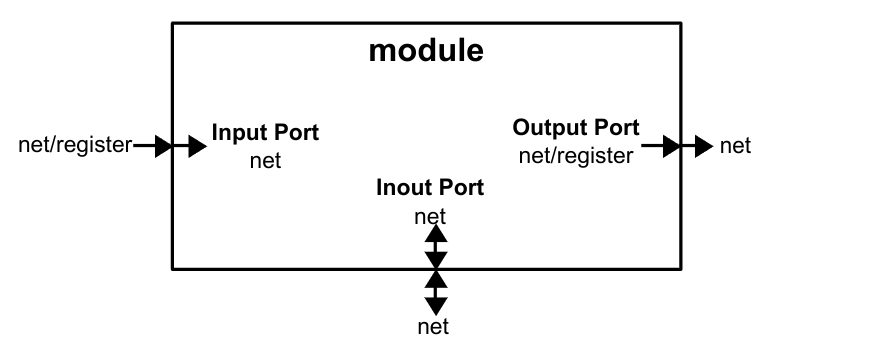
\includegraphics[width=0.7\textwidth]{img/04_nets.png}
\end{figure}

\note{
A port permits an external net or variable to connect to an internal net or variable, with restrictions.

Here are some common user errors, along with their typical error messages:
\begin{itemize}
\item We make a procedural assignment to a signal that we either declared as a net or we forgot to declare so is thus implicitly a net. This is an illegal statement.
\item We connect an output from an instance to a signal declared as a register. This is illegal as a module output can only drive a net. This is an illegal output port specification.
\item We declare a signal as a module input and as a register. This is illegal as inputs can only be nets. These are incompatible declarations.
\end{itemize}
}
\end{frame}


%%%%%%%%%%%%%%%%%%%%%%%%%%%%%%%%%%%%%%%%%%%%%%%%%%%%%%%%%%%%
\begin{frame}[fragile]
\frametitle{Net and Register Type Example}

\begin{multicols}{2}
{\tiny%
\begin{Verbatim}[commandchars=\\\{\}, tabsize=2]
\textcolor{purple}{module} yin(
	\textcolor{purple}{output reg} y_out,
	\textcolor{purple}{input wire} a_in, b_in
);
\textcolor{purple}{always} @ (a_in or b_in)
	y_out = a_in && b_in;
\textcolor{purple}{endmodule}

\textcolor{purple}{module} yang(
	\textcolor{purple}{output wire} y_out,
	\textcolor{purple}{input wire} a_in, b_in
);
\textcolor{purple}{assign} y_out <= a_in || b_in;
\textcolor{purple}{endmodule}

\textcolor{purple}{module} yin_and_yang_tb;
	\textcolor{purple}{reg} a, b;
	\textcolor{purple}{wire} and_out, or_out;
	yin u1 (and_out, a, b);
	yang u2 (or_out, a, b);
	\textcolor{purple}{initial begin}
		a = 0;
		b = 0;
		...
	\textcolor{purple}{end}
\textcolor{purple}{endmodule}
\end{Verbatim}
}

\vfill

\columnbreak

\begin{figure}[H!]
    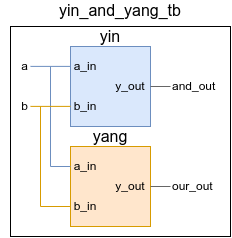
\includegraphics[width=0.45\textwidth]{img/04_net_example.png}
\end{figure}
\end{multicols}

\end{frame}

\note{
\scriptsize{
We are using here fully defined Verilog-2001 ANSI-C syntax for module port declarations for clarity.
\newline

In both module yin and yang, the input ports a\_in and b\_in \textbf{must} be declared as net data types.
\newline

In module yin, the output y\_out \textbf{must} be declared as a register data type as it is assigned from the \textit{always} procedural block.
\newline

In module yang, the output y\_out \textbf{must} be declared as a net type as it is driven from the continuous assign statement.
\newline

In module \textit{test}, a and b \textbf{must} be declared as register data types as they are assigned from the \textit{initial} procedural block, but and\_out and or\_out \textbf{must} be declared as net data types as they are driven from the instance output ports.
\newline

Therefore a connection like a -$>$ a\_in, or y\_out -$>$ and\_out actually changes data type as it crosses the module boundary.

}
}
%%%%%%%%%%%%%%%%%%%%%%%%%%%%%%%%%%%%%%%%%%%%%%%%%%%%%%%%%%%%
\begin{frame}[fragile]
\frametitle{Declaring Vectors}

A vector is a net or reg with a range specification.

We can specify the vector's range when declaring the variable:
\begin{itemize}
\item {[msb : lsb]} or {[lsb: msb]}
\item Range can be ascending or descending
\item Bounds can be negative, zero or positive
\item Bounds must be constant expressions
\item Individual bits can be selected from a vector
\end{itemize}

\begin{multicols}{2}
{\footnotesize%
\begin{Verbatim}[commandchars=\\\{\}, tabsize=2]
\textcolor{purple}{module} mux4 (
	\textcolor{purple}{input wire} [3:0] a, b,
	\textcolor{purple}{input wire}       sel,
	\textcolor{purple}{output reg} [3:0] op
);
\textcolor{purple}{always} @ (a or b or sel)
	\textcolor{purple}{if} (sel == 1)
		op = b;
	\textcolor{purple}{else}
		op = a;
\textcolor{purple}{endmodule}

\end{Verbatim}
}

\vfill

\columnbreak

\begin{figure}
    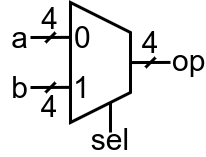
\includegraphics[width=0.40\textwidth]{img/04_vectors.png}
\end{figure}
\end{multicols}

\end{frame}

\note {
Ports, nets, and variables of the \textbf{reg} type are a single bit unless we declare them with a range.
\newline

To declare u multiple bit \textbf{port, net,} or \textbf{reg} variable, we need to specify a range. The range provides addresses for the individual bits. The only restriction on the range bounds is that they must be constant expressions. Either or both bound can be negative, zero, or positive, and the range can be ascending or descending.

}

%%%%%%%%%%%%%%%%%%%%%%%%%%%%%%%%%%%%%%%%%%%%%%%%%%%%%%%%%%%%
\begin{frame}
\frametitle{Using Vector Ranges}

Access vector selections whatever way you declared the range.
\begin{itemize}
\item Select one or more contiguous bits.
\end{itemize}
\begin{figure}[H!]
    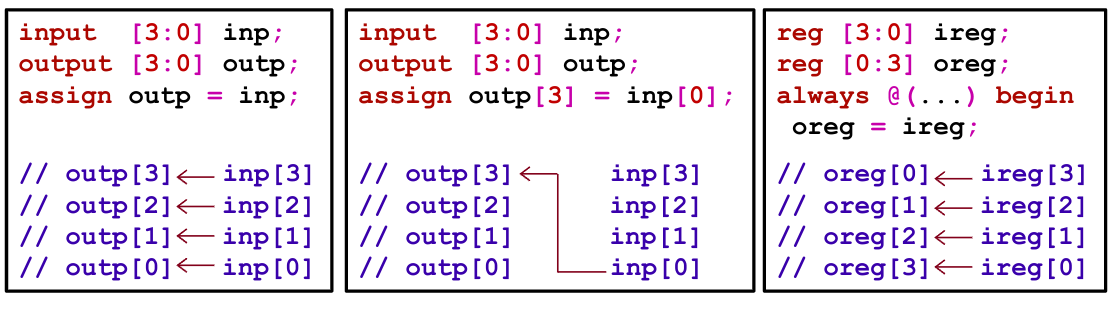
\includegraphics[width=0.95\textwidth]{img/04_range.png}
\end{figure}

\end{frame}

\note{
The vector range provides addresses for the individual bits. We can address a vector bit by providing an index and a vector part by providing a range. 
\newline

The part selection range must be in the same order as in the declaration, either ascending or descending.
\newline

The first illustration assigns an \textit{input} port to the \textit{output} port.
\newline 

The second illustration assigns one bit of an \textit{input} port to one bit of the \textit{output} port.
\newline

The third illustration assigns the value of a \textit{reg} vector to another \textit{reg} vector.

}

%%%%%%%%%%%%%%%%%%%%%%%%%%%%%%%%%%%%%%%%%%%%%%%%%%%%%%%%%%%%
\begin{frame}
\frametitle{Assigning Between Different Widths}
Vector widths do not need to match in an assignment!
\begin{itemize}
\item Source wider than target truncates value from msb.
\item Unsigned source shorter that target zero-extends value.
\item Signed source shorter that target sign-extends value.
\begin{itemize}
	\item Selections and concatenations are not considered signed.
\end{itemize}
\end{itemize}
\begin{figure}[H!]
    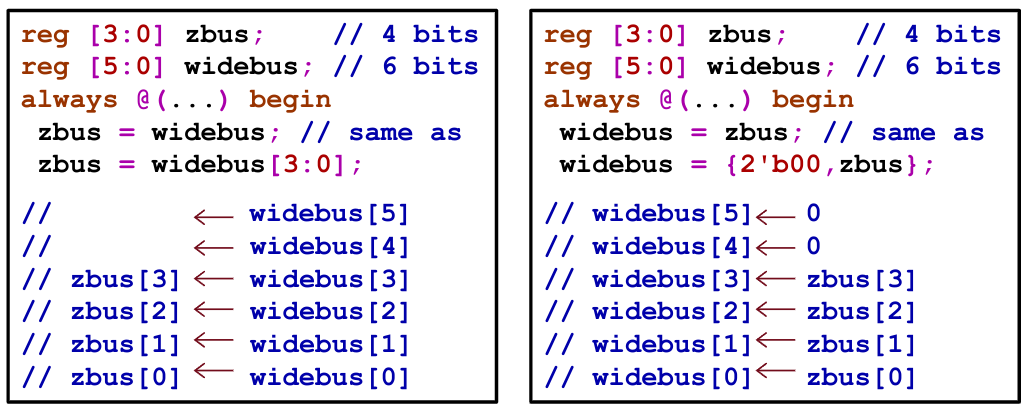
\includegraphics[width=0.95\textwidth]{img/04_width.png}
\end{figure}

\end{frame}

\note{
We can assign between vectors of different widths:
\begin{itemize}
\item Verilog truncates the leftmost bits when assigning a wider vector to a narrower vector. If we want to select some range other that the rightmost bits then you must specify that range.
\item Verilog pads the leftmost bits with 0 when assigning narrower vector to a wider vector. If you want to assign something other that 0, then you need to use the concatenation operator to construct a wider expression.
\end{itemize}
}
%%%%%%%%%%%%%%%%%%%%%%%%%%%%%%%%%%%%%%%%%%%%%%%%%%%%%%%%%%%%
\begin{frame}
\frametitle{Defining Literal Values}

We can specify a literal value as: \textcolor{red}{$<size>'<base><value>$}
\begin{itemize}
\item \textcolor{purple}{size} is an optional positive decimal number. If unsized is at least 32 bits.
\item \textcolor{purple}{base} is a character to indicate binary, octal, decimal, or hexadecimal radix.
\begin{itemize}
	\item B/b, O/o, D/d, H/h
	\item Verilog-2001: Optionally preceded by and "s" character to indicate a signed value.
\end{itemize} 
\item \textcolor{purple}{value} is legal digits for base:
\begin{itemize}
	\item Can include "\_" if not 1st character
	\item Can include Z/z and X/x if base is binary, octal or hexadecimal
	\item Verilog-2001: can be single Z/z or X/x digit if decimal base
	\item value is itself an unsigned number
\end{itemize}
\end{itemize}

\begin{figure}[H!]
    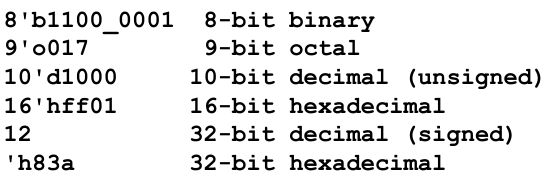
\includegraphics[width=0.55\textwidth]{img/04_literal.png}
\end{figure}

\end{frame}

\note{
\tiny{
We specify integer literals in binary, octal, decimal or hexadecimal format.
\newline

We can specify a decimal integer literal as an optional sign fallowed by a sequence of decimal digits. A number in this format is a signed number.
\newline

We can specify any integer literal as an optional sign fallowed by and optional size followed by a single quote followed by one or two base format characters and then followed by a sequence of digits appropriate to the radix.
\newline

A literal that we do not size has a size of at least 32 bits and most implementations make it exactly 32 bits.
\newline

There must be no white space between the single quote character and the base format. The base format is not sensitive to character case and consists of a \textbf{b, o, d, h} characters to indicate the radix.
\newline

The Verilog-2001 update allows an optional preceding "s" character to indicate a signed value.
\newline

The digit sequence is not sensitive to character case and consists of digits  for the radix. For the binary, octal or hexadecimal radices, we can use the "z" and "x" characters for any of the digits. The Verilog-2001 update also permits a decimal value to be a single "z" or "x" character to indicate a value that is high impedance or all unknown.
\newline

Except for the first digit, we can insert underscore "\_" characters anywhere we nedd them to improve readability. 
\newline

We can substitute the "?" character for a "z" character. This will become obvious when we study the case statement.
\newline

\textcolor{red}* Appropriately sizing the literal avoids padding and truncation!

}
}

%%%%%%%%%%%%%%%%%%%%%%%%%%%%%%%%%%%%%%%%%%%%%%%%%%%%%%%%%%%%
\begin{frame}
\frametitle{Automatic Extension of Unsigned Literals}
\scriptsize{
For \textcolor{purple}{sized literals} (e.g. 2'b11):
\begin{itemize}
\item Verilog pads to left with 0 to match size of wider expression.
\end{itemize}

For \textcolor{purple}{unsized literals} (e.g. 'b11):
\begin{itemize}
\item Size is 32 bits.
\item If leftmost digit is 1 or 0: 
\begin{itemize}
\scriptsize{
	\item Verilog left-fills to make 32 bits and pads to left with 0 to match the size of wider expression.
}
\end{itemize}
\item If leftmost digit is Z or X:
\begin{itemize}
\scriptsize{
	\item Verilog left-fills with that leftmost digit to make 32 bits.
	\item Verilog-1995 then pads to left with 0 to match size of wider expression.
	\item Verilog-2001: then pads to left with that leftmost digit to match size of wider expression.
}
\end{itemize}
\end{itemize}
}

\begin{multicols}{2}

\begin{figure}
    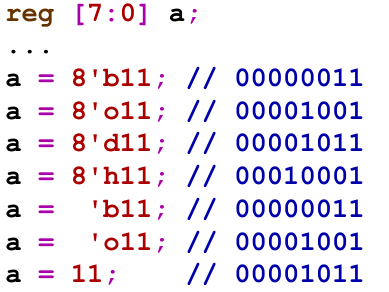
\includegraphics[width=0.35\textwidth]{img/04_ext0.png}
\end{figure}
\vfill

\columnbreak

\begin{figure}
    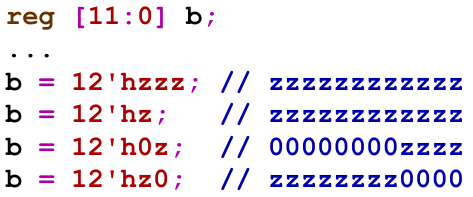
\includegraphics[width=0.45\textwidth]{img/04_ext1.png}
\end{figure}
\end{multicols}

\end{frame}

\note{
The Verilog 2001 standard permits signed based literals. The sign bit can be 0, 1, x or z. Verilog 2001 sign-extends signed based literals to match the width of the enclosing expression.
\newline

Verilog zero-extends unsigned based literals except in one situation. If the provided value has fever digits than what the size indicates and the leftmost bit is z or x, then Verilog extends the provided value with that z or x bit value up to the size of the literal. This made it easy to fill an entire vector with z or x.
\newline

The standard guarantees that the size of an unsigned literal is at least 32 bits and most implementations made it exactly 32 bits. The Verilog-2001 update continues to extend the z or x up to the width of the enclosing expression.

}

%%%%%%%%%%%%%%%%%%%%%%%%%%%%%%%%%%%%%%%%%%%%%%%%%%%%%%%%%%%%
\begin{frame}
\frametitle{Variable Vector Selection}
\begin{multicols}{2}
\scriptsize{
\textcolor{red}{Bit-select}:
\begin{itemize}
\item A single bit-select index may be variable.
\end{itemize}

\textcolor{red}{Range-select}:
\begin{itemize}
\item In Verilog-1995, range-select indices must be constant.
\item In Verilog-2001, a range-select can use a variable index and a constant width:
\begin{itemize}
\scriptsize{
	\item Base expression (variable)
	\item Width expression (constant)
	\item Offset direction:
	\begin{itemize}
		\scriptsize{
		\item Positive +
		\item Negative -
		}
	\end{itemize}
	\item Offset indicates if the width is added or substracted from the base:
}
\end{itemize}
\end{itemize}
}
\begin{figure}
    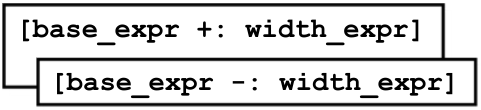
\includegraphics[width=0.45\textwidth]{img/04_offset.png}
\end{figure}
\vfill
\columnbreak

\begin{figure}
    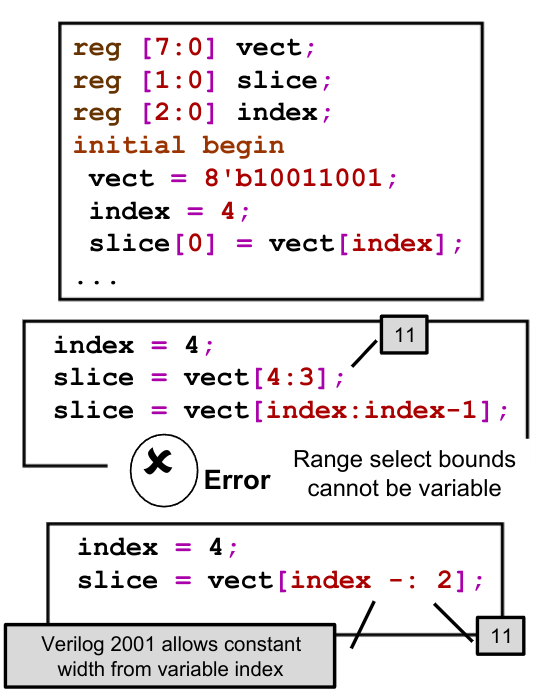
\includegraphics[width=0.45\textwidth]{img/04_selection.png}
\end{figure}
\end{multicols}

\end{frame}

\note{
\scriptsize{
Individual bits can be selected from a vector using a variable or expression index.
\newline

However in extracting a range of bits from a vector, Verilog-1995 requires that both bounds of the range are constants or constant expression. So a variable cannot be used in the extraction of a range of bits.
\newline

identifier {[msb\_constant\_expression:lsb\_constant\_expression]}
\newline

Verilog-2001 provides an alternative syntax that permits the starting point of a range select to be a variable expression, as long as the number of bits selected is a constant. In effect, to select a constant-width range from a variable starting bit position. The constant offset can be positive or negative from the starting point.
\newline

identifier {[base\_expression+:width\_constant\_expression]}
\newline
identifier {[base\_expression-:width\_constant\_expression]}
\newline

Where: \textit{base\_expression} is the variable starting bit position and \textit{width\_constant\_expression} is a constant plus or minus offset.

}
}

%%%%%%%%%%%%%%%%%%%%%%%%%%%%%%%%%%%%%%%%%%%%%%%%%%%%%%%%%%%%
\begin{frame}
\frametitle{Declaring Nets}

\end{frame}

%%%%%%%%%%%%%%%%%%%%%%%%%%%%%%%%%%%%%%%%%%%%%%%%%%%%%%%%%%%%
\begin{frame}
\frametitle{Module}

\end{frame}

%%%%%%%%%%%%%%%%%%%%%%%%%%%%%%%%%%%%%%%%%%%%%%%%%%%%%%%%%%%%
\begin{frame}
\frametitle{Module}

\end{frame}

%%%%%%%%%%%%%%%%%%%%%%%%%%%%%%%%%%%%%%%%%%%%%%%%%%%%%%%%%%%%
\begin{frame}
\frametitle{Module}

\end{frame}

%%%%%%%%%%%%%%%%%%%%%%%%%%%%%%%%%%%%%%%%%%%%%%%%%%%%%%%%%%%%
\begin{frame}
\frametitle{Module}

\end{frame}

%%%%%%%%%%%%%%%%%%%%%%%%%%%%%%%%%%%%%%%%%%%%%%%%%%%%%%%%%%%%
\begin{frame}
\frametitle{Module}

\end{frame}

%%%%%%%%%%%%%%%%%%%%%%%%%%%%%%%%%%%%%%%%%%%%%%%%%%%%%%%%%%%%
\begin{frame}
\frametitle{Module}

\end{frame}

\end{document}
